\documentclass[12pt]{article}
\usepackage{indentfirst}
\usepackage{siunitx}
\usepackage{graphicx}
\usepackage{subfigure}
\usepackage{float}
\usepackage{amsmath}
\usepackage{tikz}
\usepackage{pgfplots}
\usetikzlibrary{matrix}

% Set the overall layout of the tree
\tikzstyle{level 1}=[level distance=3.5cm, sibling distance=3.5cm]
\tikzstyle{level 2}=[level distance=3.5cm, sibling distance=2cm]

\setlength{\parindent}{20pt}
\setlength{\oddsidemargin}{0.25cm}
\setlength{\evensidemargin}{0.25cm}
\setlength{\marginparsep}{0.5cm}
\setlength{\marginparwidth}{1.5cm}
\setlength{\textwidth}{160mm}
\renewcommand{\baselinestretch}{1.5}

\pgfplotsset{compat=1.6}

\pgfplotsset{soldot/.style={color=blue,only marks,mark=*}} \pgfplotsset{holdot/.style={color=blue,fill=white,only marks,mark=*}}


\author{WU, Chenhao  117010285}
\title{CIE 6020 Assignment 3}
\date{March 2, 2019}

\begin{document}
	\maketitle
	\par 
	1. \textit{Source coding.} Let $p$ be a distribution on {$a$, $b$} with $p(a)=0.4$ and $p(b)=0.6$. Draw the curve of $M^{*}(3, \epsilon)$ for $\epsilon in [0, 1]$. Specify all the continuous points. \\
	\textbf{Answer:} \\
	We can calculate the probability of each sequence with length equal to 3.
	\begin{align*}
		p(aaa) &= 0.064 \\
		p(aab) &= p(aba) = p(baa) = 0.096 \\
		p(abb) &= p(bab) = p(bba) = 0.144 \\
		p(bbb) &= 0.216
	\end{align*}
	then we can obtain the smallest cardinality of 3-length block code with $\epsilon \in [0, 1]$
	\begin{equation}
		M^{*}(3, \epsilon) = \left\{
		\begin{array}{rcl}
		8 && {0 \leq \epsilon < 0.064} \\
		7 && {0.064 \leq \epsilon < 0.16} \\
		6 && {0.16 \leq \epsilon < 0.256} \\
		5 && {0.256 \leq \epsilon < 0.352} \\
		4 && {0.352 \leq \epsilon < 0.496} \\
		3 && {0.496 \leq \epsilon < 0.64} \\
		2 && {0.64 \leq \epsilon < 0.784} \\
		1 && {0.784 \leq \epsilon < 1} \\
		0 && {\epsilon = 1}
		\end{array}
		\right.
	\end{equation}
	Curve of $M$ can be drawn as \\
	\begin{figure}[!h]
	\centering
	\begin{tikzpicture}[scale=1.5]
	\centering
	\begin{axis}
		\addplot[domain=0:0.064,blue] {8};
		\addplot[domain=0.064:0.16,blue] {7};
		\addplot[domain=0.16:0.256,blue] {6};
		\addplot[domain=0.256:0.352,blue] {5};
		\addplot[domain=0.352:0.496,blue] {4};
		\addplot[domain=0.496:0.64,blue] {3};
		\addplot[domain=0.64:0.784,blue] {2};
		\addplot[domain=0.784:1,blue] {1};
		\addplot[soldot] coordinates{(0,8)(0.064,7)(0.16,6)(0.256,5)(0.352,4)(0.496,3)(0.64,2)(0.784,1)(1,0)};
		\addplot[holdot] coordinates{(0.064,8)(0.16,7)(0.256,6)(0.352,5)(0.496,4)(0.64,3)(0.784,2)(1,1)};
		\draw[dotted] (axis cs:0.064,8) -- (axis cs:0.064,7);
		\draw[dotted] (axis cs:0.16,7) -- (axis cs:0.16,6);
		\draw[dotted] (axis cs:0.256,6) -- (axis cs:0.256,5);
		\draw[dotted] (axis cs:0.352,5) -- (axis cs:0.352,4);
		\draw[dotted] (axis cs:0.496,4) -- (axis cs:0.496,3);
		\draw[dotted] (axis cs:0.64,3) -- (axis cs:0.64,2);
		\draw[dotted] (axis cs:0.784,2) -- (axis cs:0.784,1);
		\draw[dotted] (axis cs:1,1) -- (axis cs:1,0);
	\end{axis}	
	\end{tikzpicture}
	\end{figure}
	\par 
	
	2. \textit{Prefix codes.} Consider a probability distribution $p=(p_1,p_2,...,p_m)$ with $p_1\geq p_2\geq...\geq p_m$. Let $p^\prime=(p_1,p_2,...,p_{m-2},p_m+p_{m-1})$. What is the difference between the optimal prefix code lengths for $p$ and $p^\prime$? \\
	\textbf{Answer:} \\
	From the lower bound for prefix code we can infer that 
	\begin{align*}
		L^{*}_{p}(x) &\geq H(p) =  - \sum_{i = 1}^{m} p_i\log p_i \\
		L^{*}_{p^\prime}(x) &\geq H(p^\prime) = -\sum_{i=1}^{m-2} p_i\log p_i - (p_{m-1}+p_m)\log(p_{m-1}+p_m) 
	\end{align*}
	in which
	\begin{align*}
		p_{m-1}\log(p_{m-1}+p_m) + p_m\log(p_{m-1}+p_m) \geq p_{m-1}\log p_{m-1} + p_m\log p_m
	\end{align*}
	thus, the optimal prefix code length of $p$ is longer than $p^\prime$
	\\
	\par 
	
	3. \textit{Huffman coding.} Consider the random variable
	\[
	X =
	\begin{bmatrix}
		x_1 & x_2 & x_3 & x_4 & x_5 & x_6 & x_7 \\
		0.49 & 0.26 & 0.12 & 0.04 & 0.04 & 0.03 & 0.02
	\end{bmatrix}
	\]
	(a) Find a binary Huffman code for $X$.\\
	(b) Find the expected code length for the above encoding.\\
	\textbf{Answer:} \\
	(a) From the random distribution we can obtain a Huffman Code tree as 
	\begin{figure}[!h]
		\centering
		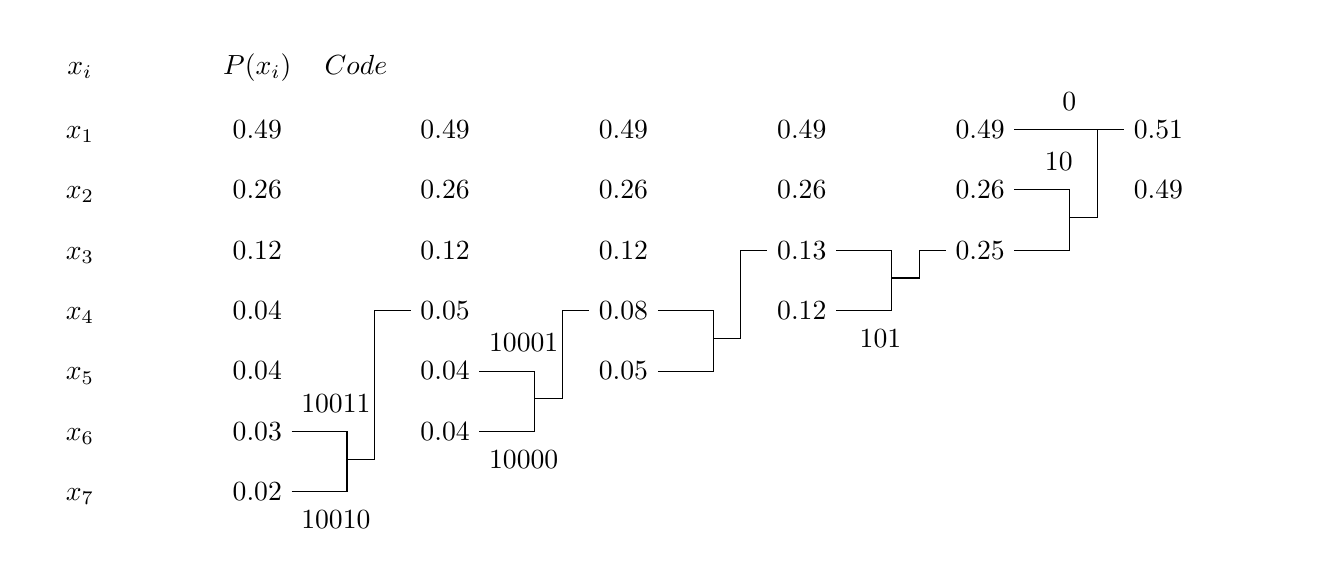
\begin{tikzpicture}
		[every node/.style={minimum height=2em}]
		\matrix [matrix of math nodes](Mat)
		{
			x_i  &|[minimum width=4em]|& P(x_i) &|[minimum width=4em]| Code &       &|[minimum width=4em]|      &       &|[minimum width=4em]|  &   &|[minimum width=4em]|  &   &|[minimum width=4em]|  &   &|[minimum width=4em]|  &   &\\			
			x_1 & & 0.49    &   & 0.49  &   & 0.49   &   & 0.49  &   & 0.49  &   &  0.51  &   & &\\
			x_2 & & 0.26    &   & 0.26  &   & 0.26   &   & 0.26  &   & 0.26  &   &  0.49  &   & &\\
			x_3 & & 0.12    &   & 0.12  &   & 0.12   &   & 0.13  &   & 0.25  &   &        &   & &\\
			x_4 & & 0.04    &   & 0.05  &   & 0.08   &   & 0.12  &   &       &   &        &   & &\\
			x_5 & & 0.04    &   & 0.04  &   & 0.05   &   &       &   &       &   &        &   & &\\
			x_6 & & 0.03    &   & 0.04  &   &        &   &       &   &       &   &        &   & &\\
			x_7 & & 0.02    &   &       &   &        &   &       &   &       &   &        &   & &\\
		};
		
		\draw (Mat-7-3.east) -|node[above,pos=0.4]{10011}++(2em,-1em) coordinate(p1) --++(1em,0) |- (Mat-5-5.west);
		\draw (Mat-8-3.east) -|node[below,pos=0.4]{10010} (p1);
		
		\draw (Mat-6-5.east) -|node[above,pos=0.4]{10001}++(2em,-1em) coordinate(p2) --++(1em,0) |- (Mat-5-7.west);
		\draw (Mat-7-5.east) -|node[below,pos=0.4]{10000} (p2);
		
		\draw (Mat-5-7.east) -|node[above,pos=0.4]{}++(2em,-1em) coordinate(p3) --++(1em,0) |- (Mat-4-9.west);
		\draw (Mat-6-7.east) -|node[below,pos=0.4]{} (p3);
		
		\draw (Mat-4-9.east) -|node[above,pos=0.4]{}++(2em,-1em) coordinate(p4) --++(1em,0) |- (Mat-4-11.west);
		\draw (Mat-5-9.east) -|node[below,pos=0.4]{101} (p4);
		
		\draw (Mat-3-11.east) -|node[above,pos=0.4]{10}++(2em,-1em) coordinate(p5) --++(1em,0) |- (Mat-2-13.west);
		\draw (Mat-4-11.east) -|node[below,pos=0.4]{} (p5);
		
		\draw (Mat-2-11.east) -- (Mat-2-11-|Mat-2-13.west)node[above,midway]{0};
		
		\end{tikzpicture}
	\end{figure}
	\\in which the Huffman coding can be listed as
	\begin{table}[H]
		\centering
		\makebox[\linewidth]{
			\begin{tabular}{|c|c|c|}
				\hline
				\textbf{Symbol} & \textbf{Codeword Length} & \textbf{Code} \\
				\hline
				$x_1$ & 1 & 0 \\ 
				\hline
				$x_2$ & 2 & 10 \\
				\hline
				$x_3$ & 3 & 101 \\
				\hline
				$x_4$ & 5 & 10001 \\
				\hline
				$x_5$ & 5 & 10000 \\
				\hline
				$x_6$ & 5 & 10011 \\
				\hline
				$x_7$ & 5 & 10010 \\
				\hline
			\end{tabular}
		}
	\end{table}
	
	(b) The expect code length can be obtained by 
	\begin{align*}
		L_f(p) &= \sum_{a\in\mathcal{A}}p(a)l(a) \\
			   &= 2.02 (bits)
	\end{align*}
	\\
	\par 
	
	4. Count the exact number of different types in $\mathcal{X}^n$, where $\mathcal{X}$ is a finite set. \\
	\textbf{Answer:} \\
	Suppose that the alphabet $\mathcal{X} = \{a_1, a_2, a_3,...,a_{|\mathcal{X}|}\}$ and $N(a|x^n)$ be the number of times that a appears in sequence $x^n$. \\
	Let $P_n$ be the collection of all possible types of sequences of length $n$.
	\begin{align*}
		P_n &= \{ (P(a_1), P(a_2),...,P(a_{|\mathcal{X}|}))\}
	\end{align*}
	where $N(a_0) + N(a_1) + N(a_2) + ... + N(a_{|\mathcal{X})|}) = n$, thus $|P_n| = \binom{n+2}{|\mathcal{X}|-1}$
	\\
	\par 
	
	5. Let $p$ be any probability distribution over a finite set $\mathcal{X}$ and $c$ be a real number in $(0, 1)$. Prove that for any subset $A$ of $\mathcal{X}^n$ with $p^n(A) \geq c$ and sufficiently large $n$, 
	\begin{align*}
		|A\cap T^n_{[X]\delta}| \geq 2^{n(H(p)-\delta^\prime)}
	\end{align*}
	where $\delta^\prime \rightarrow 0$ as $\delta \rightarrow 0$. \\
	\textbf{Proof:} \\
	The probability that an n-length sequence \textbf{x} in subset A can be generated as
	\begin{align*}
		p^n(\textbf{X}^n\in A\cap T_{[X]\delta}^n) &= \sum_{x\in A\cap T_{[X]\delta}^n} p^n(x)\\
												   &\leq \sum 2^{-nH(p) - nD(p||A)} \\
												   &= \sum 2^{-nH(p) - n\sum_{x^n\in\mathcal{X}^n}p^n(x^n)\log\frac{p^n(x^n)}{p^n(A)}} \\
												   &\leq \sum 2^{-nH(p) +nc} \\
												   &= |A\cap T_{[X]\delta}^n | 2^{-nH(p)+nc}
	\end{align*}
	Also, from De Morgan's law and \textbf{AEP} II, we can obtain that 
	\begin{align*}
		1 &\geq p^n(\textbf{X}^n\in A\cap T_{[X]\delta}^n)\\
		  &= 1 - p^n(\textbf{X}^n \not\in A) - p^n(\textbf{X}^n \not\in T_{[X]\delta}^n) \\
		  &\geq 1 - (1 - c) - \delta \\
		  &= c - \delta
	\end{align*}
	Combine two inequalities we can derivative that 
	\begin{align*}
		|A\cap T_{[X]\delta}^n| &\geq (c - \delta)2^{nH(p)-nc} \\
								&= 2^{nH(p) - nc + \log(c-\delta)} \\
								&= 2^{n(H(p) - c(1-\frac{\log (c-\delta)}{nc}))}
	\end{align*} 
	Let $\delta^\prime = c(1 - \frac{log(c-\delta)}{nc})$, from weak typicality we can infer that when n is sufficiently large c converges to 0 and thus, $\delta^\prime \rightarrow 0$ when $\delta \rightarrow 0$.
	
\end{document}